%
% This is the LaTeX template file for lecture notes for CS294-8,
% Computational Biology for Computer Scientists.  When preparing 
% LaTeX notes for this class, please use this template.
%
% To familiarize yourself with this template, the body contains
% some examples of its use.  Look them over.  Then you can
% run LaTeX on this file.  After you have LaTeXed this file then
% you can look over the result either by printing it out with
% dvips or using xdvi.
%
% This template is based on the template for Prof. Sinclair's CS 270.

\documentclass[twoside]{ctexart}

\usepackage{listings,xcolor}
\usepackage{enumitem}
\usepackage{mathrsfs}
\usepackage{indentfirst} 
\usepackage{lstcustom}
\usepackage{ctex}
\usepackage{comment}
\usepackage{booktabs}
\usepackage{graphicx}
\usepackage{multirow}
\usepackage{diagbox}
\usepackage{amsmath,amsfonts,graphicx,amssymb,bm,amsthm}
\usepackage{algorithm,algorithmicx}
\usepackage[noend]{algpseudocode}
\usepackage{fancyhdr}
\usepackage{tikz}
\usepackage{graphicx}
\usetikzlibrary{arrows,automata}
\usepackage{hyperref}

\setlength{\oddsidemargin}{0.25 in}
\setlength{\evensidemargin}{0.25 in}
\setlength{\topmargin}{-0.6 in}
\setlength{\textwidth}{6.5 in}
\setlength{\textheight}{8.5 in}
\setlength{\headsep}{0.75 in}
\setlength{\parindent}{0 in}
\setlength{\parskip}{0.1 in}

%
% The following commands set up the lecnum (lecture number)
% counter and make various numbering schemes work relative
% to the lecture number.
%
\newcounter{lecnum}
\newcounter{counter_exm}\setcounter{counter_exm}{1}
\newtheorem{theorem}{\hskip 1.7em 定理}
\newtheorem{lemma}[theorem]{\hskip 1.7em 引理}
\newtheorem{proposition}[theorem]{Proposition}
\newtheorem{claim}[theorem]{\hskip 1.7em 命题}
\newtheorem{corollary}[theorem]{\hskip 1.7em 推论}
\newtheorem{definition}[theorem]{\hskip 1.7em 定义}

\renewcommand{\emph}[1]{\begin{kaishu}#1\end{kaishu}}

\newenvironment{solution}{{\noindent\hskip 2em \bf 解 \quad}}


\renewenvironment{proof}{{\noindent\hskip 2em \bf 证明 \quad}}{\hfill$\qed$\par}
\newenvironment{example}{{\noindent\hskip 2em \bf 例 \arabic{counter_exm}\quad}}{\addtocounter{counter_exm}{1}\par}

\newenvironment{concept}[1]{{\bf #1\quad} \begin{kaishu}} {\end{kaishu}\par}

\newcommand\E{\mathbb{E}}

%
% The following macro is used to generate the header.
%

\newcommand{\lecture}[4]{
   \pagestyle{myheadings}
   \thispagestyle{plain}
   \newpage
   \setcounter{lecnum}{#1}
   \setcounter{page}{1}
   \noindent
   \begin{center}
   \framebox{
      \vbox{\vspace{2mm}
    \hbox to 6.28in { {\bf ICS小班课
                        \hfill 2020年秋季} }
       \vspace{4mm}
       \hbox to 6.28in { {\Large \hfill 专题#1:#2  \hfill} }
       \vspace{2mm} 
       \hbox to 6.28in { {\it  \hfill 作者:#3} }
      \vspace{2mm}}
   }
   \end{center}
   \markboth{专题#1:#2}{专题#1:#2}
   {\bf 免责声明}:{\it 该笔记尚未进行正式出版物的通常审查,未经教师允许不能向课程外分发.}
   \vspace*{4mm}
}


\renewcommand{\cite}[1]{[#1]}
\def\beginrefs{\begin{list}%
        {[\arabic{equation}]}{\usecounter{equation}
         \setlength{\leftmargin}{2.0truecm}\setlength{\labelsep}{0.4truecm}%
         \setlength{\labelwidth}{1.6truecm}}}
\def\endrefs{\end{list}}
\def\bibentry#1{\item[\hbox{[#1]}]}

%Use this command for a figure; it puts a figure in wherever you want it.
%usage: \fig{NUMBER}{SPACE-IN-INCHES}{CAPTION}
\newcommand{\fig}[3]{
			\vspace{#2}
			\begin{center}
			图 \thelecnum.#1:~#3
			\end{center}
	}

% **** IF YOU WANT TO DEFINE ADDITIONAL MACROS FOR YOURSELF, PUT THEM HERE:
\DeclareMathOperator*{\argmax}{\arg\max}
\DeclareMathOperator*{\argmin}{\arg\min}

\begin{document}

% title 
\lecture{0}{Latex介绍}{杨晨阳}


    \section{如何在Overleaf上使用本模板?}
    
    在左侧点击New File图标,新建文件LecX.tex,其中X是课次,将本模板复制进去。填写需要填写的信息,清空正文部分,就可以开始写了。
    
    如果是在本地编译:编译采用的是Xe\LaTeX ,本地编译采用pdf\LaTeX 可能失败。
    
    \section{如何插入图片?}
    
    使用figure环境,[ \quad ]内的字母表示可以使用的图片插入位置选择。
    h代表放在当前位置,t代表放在顶部,b代表放在底部,三者顺序表示三个准则的优先级。比如下面'htb'的组合表示优先放在当前位置,如果放不下,那就放在下一页的头部,再不然则放在底部。
    
    \begin{figure}[htb]
        \centering
        % width 指想要把插入后的图片调整到多大,我这里设定的是0.3倍
        % 行宽度(\textwidth)
        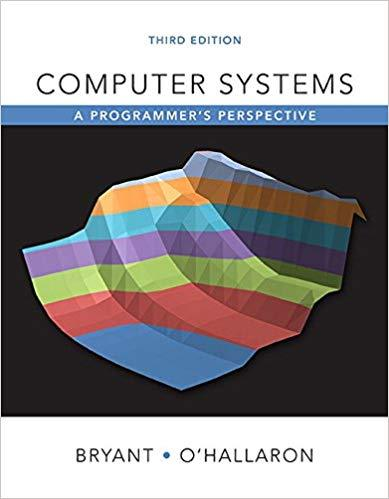
\includegraphics[width = 0.3\textwidth]{figure/csapp.jpg}
        \caption{Csapp 0.3倍大}
        \label{fig:my_label}
    \end{figure}
    
    上面的插入方式是为了满足Latex的美感,但是当连续插入多张图片时会导致图片大量窜位,影响阅读。如果想要强制固定图片和文字的位置,可以使用H,但这样有时候会出现大量空白。
    \begin{figure}[H]
        \centering
        % width 指想要把插入后的图片调整到多大,我这里设定的是0.5倍
        % 行宽度(\textwidth)
        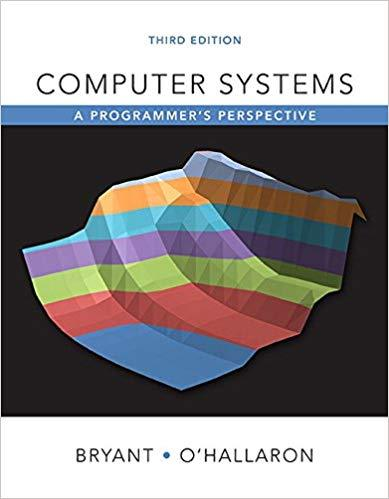
\includegraphics[width = 0.5\textwidth]{figure/csapp.jpg}
        \caption{Csapp 0.5倍大}
        \label{fig:my_label}
    \end{figure}
    
    \section{如何插入表格?}
    
    简单的表格只需要用tabular环境就可以了
    \begin{table}[H] % 表格外层的环境,没什么用
        \centering % 表示后面的居中
        \begin{tabular}{cc} 
        
        % {}中的字母数代表表格的栏数
        % cc表示都居中,cl表示第一栏居中,第二栏左对齐,类似的还有cr
        
        a & b \\ % \\ 换行, & 表示一列结束开始下一列
        c & d
        
        \end{tabular}
        \caption{一个最简单的表格}
        \label{tab:my_label}
    \end{table}
    
    不过这样的表格是没有线的,加上竖线的方法是在cc之间加入|变成c|c。这表示两列之间有竖线。|c|c|表示两列的两边也有竖线。
    
    \begin{table}[H] % 表格外层的环境,没什么用
        \centering % 表示后面的居中
        \begin{tabular}{|c|c|} 
        
        a  & b \\ 
        c  & d
        \end{tabular}
        \caption{带竖线的表格}
        \label{tab:my_label}
    \end{table}
    
    如何加入横线呢?方法是给每行加上上划线hline,这样看起来就是有横线了。(注意还要在多加一空白行来弄出最后一行内容的下划线)
    
    \begin{table}[H] % 表格外层的环境,没什么用
        \centering % 表示后面的居中
        \begin{tabular}{|c|c|} 
        \hline
        a  & b \\ 
        \hline
        c  & d \\
        \hline
        \end{tabular}
        \caption{带横线的表格}
        \label{tab:my_label}
    \end{table}
    
    不过有时候我们需要打很大的表格,这样打肯定没有excel方便,我们可以用工具把excel转成latex,下表使用的工具是excel2latex,其压缩包已放置在tools文件夹里。解压后将xla拖拽至excel里,可在加载项中找到其位置。(细节可以自行百度)

    
    \section{如何插入代码?}
    这里我们只给出一个比较麻烦的实现,大家可以自己搜索一下其他的实现。这个方案的麻烦之处在于这个实现允许自己调整配色方案,整个代码由frame构成,第一部分lstset是在设置颜色,basicstyle是正常语句的颜色,后面还可以设置字符串,关键词,背景颜色。如果设置的颜色不合心意还可以通过rgb自定义颜色(definecolor)
    
    比如下面的深色配色方案
\begin{frame}

\definecolor{darkwhite}{rgb}{0.8,0.8,0.8}
\definecolor{lightgreen}{rgb}{0,0.8,0}
\lstset{language=C++,
                basicstyle=\color{darkwhite},
                backgroundcolor = \color{black},
                keywordstyle=\color{blue}\ttfamily,
                stringstyle=\color{lightgreen}\ttfamily,
                commentstyle=\color{gray}\ttfamily,
                morecomment=[l][\color{magenta}]{\#}
}

\begin{lstlisting}
    #include<stdio.h>
    #include<iostream>
    // A comment
    int main(void)
    {
    printf("Hello World\n");
    return 0;
    }
\end{lstlisting}

\end{frame}

和下面的浅色配色方案
\begin{frame}

\definecolor{lightgreen}{rgb}{0,0.8,0}
\definecolor{darkgreen}{rgb}{0,0.8.0.2}
\lstset{language=C++,
                basicstyle=\ttfamily,
                backgroundcolor = \color{white},
                keywordstyle=\color{blue}\ttfamily,
                stringstyle=\color{lightgreen}\ttfamily,
                commentstyle=\color{gray}\ttfamily,
                morecomment=[l][\color{darkgreen}]{\#}
}
\begin{lstlisting}
    #include<stdio.h>
    #include<iostream>
    // A comment
    int main(void)
    {
    printf("Hello World\n");
    return 0;
    }
\end{lstlisting}

\end{frame}
    
    \section{如何优雅地书写定理、定义、证明?}
    
    使用以下常用的环境:
    
    % 使用环境theorem给出定理(以及corollary表示推论、claim表示断言)
    \begin{theorem}
    	\[
            (1+x)^\alpha=\sum_{n\geq 0}{\binom{\alpha}{n}}x^n.
        \]
    \end{theorem}

    % 使用环境proof给出证明
	\begin{proof}
	    $$
            \sum_{k=0}^{l} \binom{n}{k} \binom{m}{l-1} = { \binom{n+m}{l} }.
        $$
	\end{proof}
	
	% 使用环境definition给出定义
	\begin{definition}
		$n^{\underline{m}}:=n(n-1)\cdots (n-m+1)$.
	\end{definition}

    % 使用环境example给出例子
	\begin{example}
		$n$对夫妇围着一个圆桌共进晚餐,要求夫妻必须相邻,试问共有多少种不同的就坐方式?
	\end{example}
	
	\section{如何描述算法?}

    \begin{algorithm}
    \caption{Euclid algorithm}
    \label{alg:euclid}
    \begin{algorithmic}[1]
        \Procedure{Euclid}{$a,b$}\Comment{The gcd of $a$ and $b$}
        \State $r\gets a\bmod b$
        \While{$r\not=0$}
        \State $a\gets b$
        \State $b\gets r$
        \State $r\gets a\bmod b$
        \EndWhile\label{euclidendwhile}
       \State \textbf{return} $b$
       \EndProcedure
   \end{algorithmic}
   \end{algorithm}
    
    \section*{比较重要的\LaTeX 的知识之一}

    epsilon的两个打法:$\varepsilon$ vs $\epsilon$

    phi的两个打法:$\varphi$ vs $\phi$
    
    pi的两个打法:$\varpi$ vs $\pi$

    \section*{比较重要的\LaTeX 的知识之二}
    
    比较一下下面几组数学公式:
    
    $\Pr[D can distinguish O from random oracles]$ 与 $\Pr[D\text{ can distinguish }O\text{ from random oracles}]$

    $\Pr[D\text{ can distinguish }O\text{ from random oracles}]$ 与 $\Pr[D\mathrm{ can distinguish }O\mathrm{ from random oracles}]$

    $q_{fail}$ 与 $q_{\mathrm{fail}}$ (或者$q_{\text{fail}}$)

    \textit{$q_{\mathrm{fail}}$} \textit{$q_{\text{fail}}$}
    
    所以
    
    \begin{enumerate}
        \item 公式环境下如果出现普通文本的话,要用$\text{text}$或者$\mathrm{mathrm}$包起来。
        \item $\mathrm{m a t h r m}$会吃掉你的空格,但是$\text{t e x t}$不会。
        \item 当然可以在$\mathrm{m~a~t~h~r~m}$里和正常公式环境一样用波浪线代表空格。
        \item 如果是在斜体环境下,公式里原本正体的\textit{$\text{text}$}会变成斜的,但是\textit{$\mathrm{mathrm}$}就不会。
    \end{enumerate}
    
    考虑到不少会议论文模板里,theorem环境下都是斜体的,所以这里的建议是在公式里用$\mathrm{mathrm}$(尤其是在用newcommand定义一些记号的时候)。
    
    \textbf{注:} 考虑到ics内容基本不涉及数学公式,上面的大家看看就好
    
    
    \section{还有其它问题?}
    
    请联系助教


\end{document}




